\documentclass[tikz]{standalone}
\usepackage{tikz}


\begin{document}
%% 基本网格
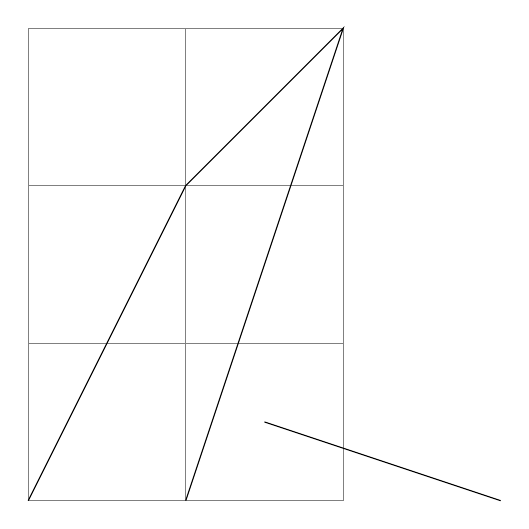
\begin{tikzpicture}[scale=2]
\draw[help lines] (0,0) grid (2,3);
\draw (0,0) --(1,2) -- (2,3) -- (1,0);
\draw (3, 0) -- (1.5, 0.5);
\end{tikzpicture}

%% 射线
\begin{tikzpicture}[scale=1]
\draw[->] (0,0) -- (2,0);
\draw[-<] (-3,1) -- (3,1);
\draw[|->] (1,2) -- (2,2);
\end{tikzpicture}

%% 两根射线连接,末端箭头
\begin{tikzpicture}
\draw[<->] (0,2)--(0,0)--(3,0);
\end{tikzpicture}

%% 更改粗细
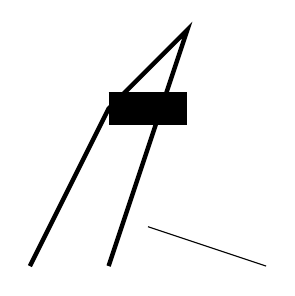
\begin{tikzpicture}[scale=1]
\draw [ultra thick](0,0) --(1,2) -- (2,3) -- (1,0);
\draw [thin](3, 0) -- (1.5, 0.5);
\draw [line width=12] (1,2) -- (2,2);
\end{tikzpicture}

%% 短线虚线,点虚线
\begin{tikzpicture}
\draw [dashed, ultra thick] (0,1) -- (2,1);
\draw [dashed] (0, 0.5) -- (2,0.5);
\draw [dotted] (0,0) -- (2,0);
\end{tikzpicture}

%% 更改颜色
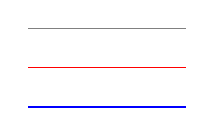
\begin{tikzpicture}
\draw [gray] (0,1) -- (2,1);
\draw [red] (0, 0.5) -- (2,0.5);
\draw [blue] (0,0) -- (2,0);
\end{tikzpicture}

%% 行内的tikz元素(失败)
wherever 

\begin{tikzpicture} 
\draw [yellow, line width=6] (0, 0)--(.5, 0); 
\end{tikzpicture} 
you want

%% 曲线
%% 矩形,圆,圆弧
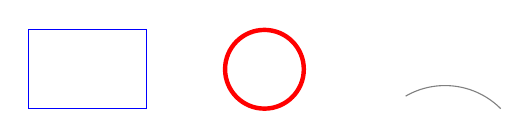
\begin{tikzpicture}
\draw [blue] (0,0) rectangle (1.5,1);
\draw [red, ultra thick] (3,0.5) circle [radius=0.5];;
\draw [gray] (6,0) arc [radius=1, start angle=45, end angle= 120];
\end{tikzpicture}
%% 圆角连接
\begin{tikzpicture}
\draw [<->, rounded corners, thick, purple] (0,2) -- (0,0) -- (3,0);
\end{tikzpicture}
%% 一个很复杂的曲线,点坐标由外部程序计算好再贴进来
\begin{tikzpicture}[xscale=25,yscale=5]
\draw [<->, help lines] (0.6,1.34) -- (0.6,1) -- (1.05,1);
\draw[orange] (0.6, 1.0385) --
(0.61, 1.06372) -- (0.62, 1.08756) -- (0.63, 1.11012) -- (0.64,
1.13147) -- (0.65, 1.15166) -- (0.66, 1.17074) -- (0.67, 1.18874) -- (0.68,
1.20568) -- (0.69, 1.22157) -- (0.7, 1.23643) -- (0.71, 1.25026) -- (0.72,
1.26307) -- (0.73, 1.27486) -- (0.74, 1.28561) -- (0.75, 1.29534) -- (0.76,
1.30402) -- (0.77, 1.31165) -- (0.78, 1.31821) -- (0.79, 1.32369) -- (0.8,
1.32806) -- (0.81, 1.33131) -- (0.82, 1.3334) -- (0.83, 1.33431) -- (0.84,
1.334) -- (0.85, 1.33244) -- (0.86, 1.32956) -- (0.87, 1.32533) -- (0.88,
1.31966) -- (0.89, 1.3125) -- (0.9, 1.30373) -- (0.91, 1.29325) -- (0.92,
1.2809) -- (0.93, 1.26649) -- (0.94, 1.24976) -- (0.95, 1.23032) -- (0.96,
1.2076) -- (0.97, 1.18065) -- (0.98, 1.14763) -- (0.99, 1.1038) -- (0.991,
1.09836) -- (0.992, 1.09261) -- (0.993, 1.0865) -- (0.994, 1.07994) -- (0.995,
1.07282) -- (0.996, 1.06497) -- (0.997, 1.0561) -- (0.998, 1.04563) -- (0.999,
1.03209) -- (0.9991, 1.03042) -- (0.9992, 1.02866) -- (0.9993,
1.02679) -- (0.9994, 1.02478) -- (0.9995, 1.0226) -- (0.9996, 1.02019) -- (0.9997,
1.01747) -- (0.9998, 1.01424) -- (0.9999, 1.01005) -- (0.9999,
1.01005) -- (0.99991, 1.00953) -- (0.99992, 1.00898) -- (0.99993,
1.0084) -- (0.99994, 1.00778) -- (0.99995, 1.0071) -- (0.99996,
1.00634) -- (0.99997, 1.00549) -- (0.99998, 1.00448) -- (0.99999, 1.00317) -- (1,
1) ;
\end{tikzpicture}

%% 指定曲线的发出和收进来的角度
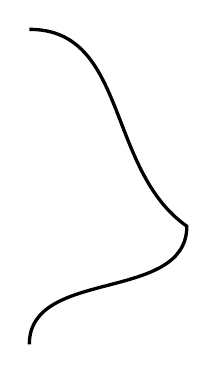
\begin{tikzpicture}
\draw[very thick] (0, 0) to [out=90, in=270] (2, 1.5) to [out=145, in=0] (0, 4);
\end{tikzpicture}

%% 绘制函数曲线 基本格式是 plot (\x, {function})
\begin{tikzpicture}[xscale=10,yscale=10]
\draw [<->] (0,0.8) -- (0,0) -- (0.5,0);
\draw[green, ultra thick, domain=0:0.5] plot (\x, {0.025+\x+\x*\x});
\end{tikzpicture}

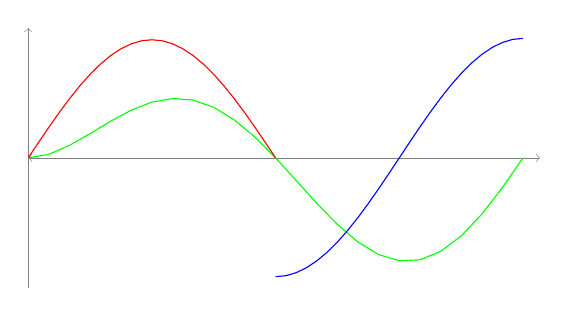
\begin{tikzpicture}[yscale=1.5]
\draw [help lines, <->] (0,0) -- (6.5,0);
\draw [help lines, ->] (0,-1.1) -- (0,1.1);
\draw [green,domain=0:2*pi] plot (\x, {(sin(\x r)* ln(\x+1))/2});
\draw [red,domain=0:pi] plot (\x, {sin(\x r)});
\draw [blue, domain=pi:2*pi] plot (\x, {cos(\x r)*exp(\x/exp(2*pi))});
\end{tikzpicture}

%% 填充区域
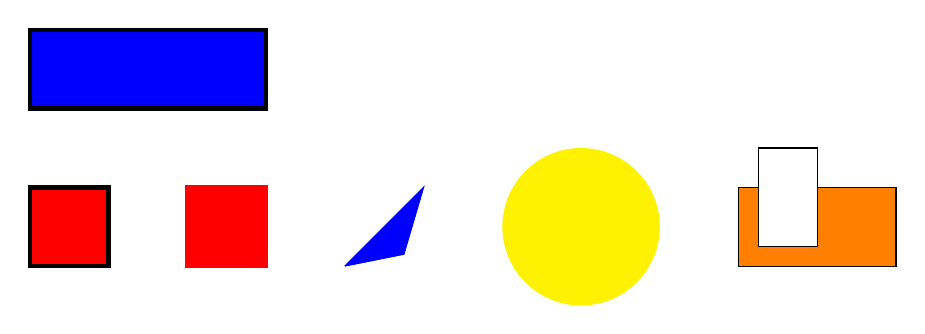
\begin{tikzpicture}
\draw [fill=red,ultra thick] (0,0) rectangle (1,1);
\draw [fill=blue,ultra thick] (0,2) rectangle (3,3);
\draw [fill=red,ultra thick,red] (2,0) rectangle (3,1);
\draw [blue, fill=blue] (4,0) -- (5,1) -- (4.75,0.15) -- (4,0);
\path [fill=yellow] (7,0.5) circle [radius=1];
\draw [fill=orange] (9,0) rectangle (11,1);
\draw [fill=white] (9.25,0.25) rectangle (10,1.5);
\end{tikzpicture}


\begin{tikzpicture}
\path [fill=gray] (0,0) rectangle (1.5,1);
\draw [fill=yellow] (2,0) rectangle (3.5,1);
\end{tikzpicture}

%% 不规则封闭路径填充
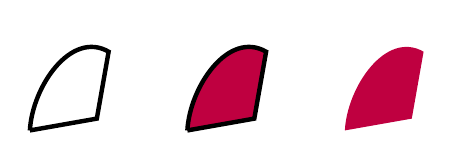
\begin{tikzpicture}
\draw [ultra thick] (0,0) to [out=87,in=150] (1,1) -- (.85,.15) -- (0,0);
\draw [ultra thick, fill=purple] (2,0) to [out=87,in=150] (3,1) -- (2.85,.15) -- (2,0);
\path [fill=purple] (4,0) to [out=87,in=150] (5,1) -- (4.85,.15) -- (4,0);
\end{tikzpicture}

%% 图中放标签
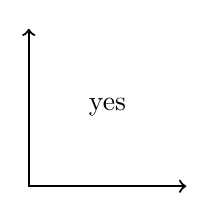
\begin{tikzpicture}
\draw [thick, <->] (0, 2) -- (0, 0) -- (2, 0);
\node at (1, 1) {yes};
\end{tikzpicture}

%% 设置标签的基准点,上面是默认baseline的位置为所设点
%% 也可以设置其他锚点位置,或者说是标签在点的那个位置
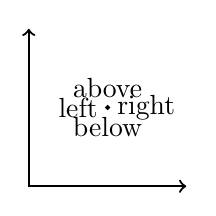
\begin{tikzpicture}
\draw [thick, <->] (0,2) -- (0,0) -- (2,0);
\draw[fill] (1,1) circle [radius=0.025];
\node [below] at (1,1) {below};
\node [above] at (1,1) {above};
\node [left] at (1,1) {left};
\node [right] at (1,1) {right};
\end{tikzpicture}

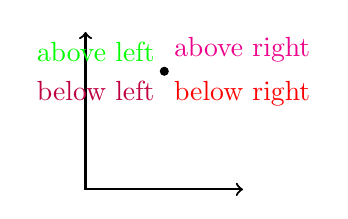
\begin{tikzpicture}[scale=2]
\draw [thick, <->] (0,1) -- (0,0) -- (1,0);
\draw[fill] (.5, .75) circle [radius=0.025];
\node [below right, red] at (.5,.75) {below right};
\node [above left, green] at (.5,.75) {above left};
\node [below left, purple] at (.5,.75) {below left};
\node [above right, magenta] at (.5,.75) {above right};
\end{tikzpicture}

%% 画坐标轴标签
\begin{tikzpicture}[xscale=1, yscale=1]
\draw [thick, <->] (0,1) -- (0,0) -- (1,0);
\node [below right] at (1, 0) {$x$};
\node [left] at (0, 1) {$y$};
\node[above left] at (1, 1) {$A$};
\draw[fill] (1, 1) circle [radius=.5pt];
\end{tikzpicture}

%% 把标签和画线语句合成一句的写法
\begin{tikzpicture}[xscale=3, yscale=3]
\draw [thick, <->] (0,1) node [left] {$y$}
-- (0,0) -- (1,0) node [below right] {$x$};
\draw[fill] (.4,.6) circle [radius=.5pt]
node[above left] {$A$};
\end{tikzpicture}

%% 标签里的文字换行写法,需要制定换行符以及对齐方式
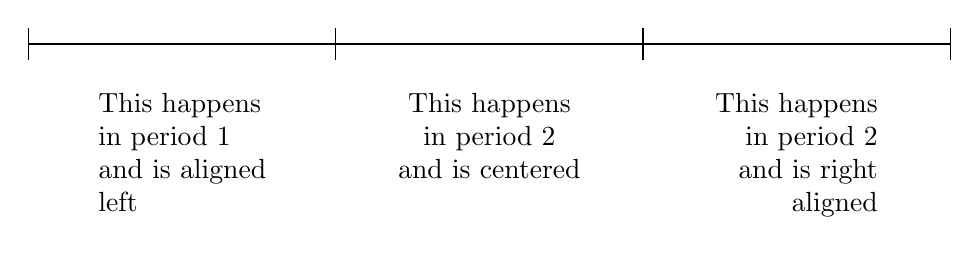
\begin{tikzpicture}[xscale=1.3]
\draw [thick] (0,0) -- (9,0);
\draw (0,-.2) -- (0, .2);
\draw (3,-.2) -- (3, .2);
\draw (6,-.2) -- (6, .2);
\draw (9,-.2) -- (9, .2);
\node[align=left, below] at (1.5,-.5)%
{This happens\\in period 1\\and is aligned\\ left};
\node[align=center, below] at (4.5,-.5)%
{This happens\\in period 2\\and is centered};
\node[align=right, below] at (7.5,-.5)%
{This happens\\in period 2\\and is right\\aligned};
\end{tikzpicture}

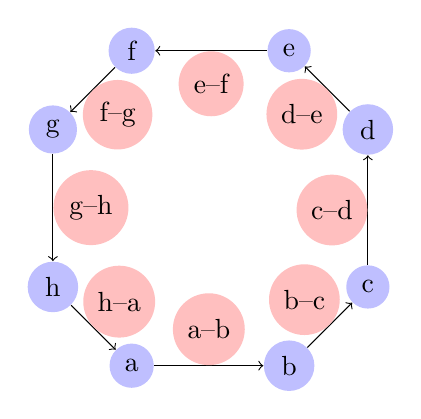
\begin{tikzpicture}  
[scale=1,auto=left,every node/.style={circle,fill=blue!25}]  
\node (a) at (-1,-2) {a};  
\node (b) at ( 1,-2) {b};  
\node (c) at ( 2,-1) {c};  
\node (d) at ( 2, 1) {d};  
\node (e) at ( 1, 2) {e};  
\node (f) at (-1, 2) {f};  
\node (g) at (-2, 1) {g};  
\node (h) at (-2,-1) {h};  
\foreach \from/\to in {a/b,b/c,c/d,d/e,e/f,f/g,g/h,h/a}  
\draw [->] (\from) -- (\to)  
node[midway,fill=red!25] {\from--\to};  
\end{tikzpicture}  
\end{document}